\documentclass[11pt]{article}
\usepackage[margin=1in]{geometry}
\usepackage{graphicx, booktabs, hyperref, xcolor, amsmath}

\begin{document}

\begin{center}
{\Large \textbf{Experiment Results:\\Bilateral Asymmetric Information Bargaining (Baseline)}}\\[0.5em]
{\large \today \quad $\cdot$ \quad Status: Post-analysis}
\end{center}

%% --- 1. RESEARCH QUESTION ---
\section*{Research Question}

Under bilateral asymmetric information, do LLM-simulated bargaining agents reach efficient deals, and does the agreed price reflect each party's private information as standard theory predicts?

In this game, a buyer (simulated human, \texttt{gpt-5-nano}) and an AI seller (\texttt{gpt-5}) negotiate over an item via alternating offers. Each party knows only their own private value: the buyer knows their valuation $v \in \{60, 70, 80, 90\}$ but not the seller's cost $c \in \{20, 30, 40, 50\}$, and vice versa. Both know the opponent's value is uniform over the four-element set. The zone of possible agreement (ZOPA) is always positive ($v - c \in [10, 70]$, mean $= \$43.50$), so efficient deals are always feasible.

The baseline prediction from standard Bayesian bargaining theory is: (1) deal rates near 100\% given large ZOPAs; (2) deal prices that increase in buyer value (buyers with higher surplus can concede more) and in seller cost (sellers with higher cost demand more); (3) deal prices close to the Nash bargaining solution (midpoint of ZOPA). No hypothesis memo exists for this game --- this is a baseline characterization of LLM behavior under bilateral asymmetric information.

%% --- 2. EXPERIMENTAL DESIGN ---
\section*{Experimental Design}

\textbf{Game structure.} Single condition (no between-subjects manipulation). The buyer offers on odd rounds (1, 3, 5); the AI offers on even rounds (2, 4). Maximum 5 rounds; no deal yields \$0 for both. Parameters are randomized per session: $v$ and $c$ drawn independently and uniformly from their respective sets.

\begin{table}[h!]
\centering
\begin{tabular}{@{}lll@{}}
\toprule
Variable & Values & Type \\
\midrule
\texttt{buyer\_value} ($v$) & \$60, \$70, \$80, \$90 & Randomized per session \\
\texttt{seller\_cost} ($c$) & \$20, \$30, \$40, \$50 & Randomized per session \\
\texttt{zopa} & $v - c$ & Derived \\
\texttt{fair\_price} & $(v + c)/2$ & Derived (midpoint) \\
\bottomrule
\end{tabular}
\caption{Game variables. All four buyer values and all four seller costs are possible in each session.}
\end{table}

\noindent\textbf{Sample.} $N = 20$ sessions run with \texttt{interview simulate bargain\_asymmetric -n 20}. Design: random assignment (not factorial), yielding unequal cell counts across the 16 parameter combinations.

%% --- 3. DATA OVERVIEW ---
\section*{Data Overview}

\textbf{Sample.} $N = 20$ sessions total. Condition distribution: \texttt{buyer\_value} ranged from 4 sessions at \$60 to 9 at \$70 (unbalanced due to random draw). \texttt{seller\_cost} ranged from 2 sessions at \$50 to 8 at \$20. ZOPA range: \$20--\$70, mean $= \$43.50$.

\textbf{Checker results.} 19/20 nominal pass (95\%). One session (\texttt{sim13}) failed the checker; inspection shows a checker false positive on arithmetic (human earns \$10 = \$60 $-$ \$50, which is correct). No substantive game failures were detected.

\begin{table}[h!]
\centering
\begin{tabular}{@{}lrr@{}}
\toprule
Metric & Value & SD \\
\midrule
Deal rate & 100\% ($N=20$) & --- \\
Mean deal price & \$54.60 & \$5.96 \\
Mean fair price (midpoint) & \$51.75 & \$7.29 \\
Price deviation from fair & $+\$2.85$ & --- \\
Mean human earnings & \$18.40 & \$10.64 \\
Mean AI earnings & \$25.10 & \$13.40 \\
Buyer surplus share & 0.450 & 0.260 \\
Mean rounds to deal & 4.30 & 1.23 \\
First offer (buyer) & \$50.00 & \$5.00 \\
\bottomrule
\end{tabular}
\caption{Summary statistics across all 20 sessions.}
\end{table}

%% --- 4. RESULTS ---
\section*{Results}

\subsection*{Primary Outcome: Deal Rate}

All 20 sessions reached a deal (100\%). This confirms that large ZOPAs (mean $= \$43.50$) make efficient agreement readily achievable even under bilateral asymmetric information, consistent with the theoretical baseline.

\subsection*{Deal Price and Surplus Split (Figure~\ref{fig:price})}

The mean deal price was \$54.60 (SD $= \$5.96$), versus a mean fair-price midpoint of \$51.75 (SD $= \$7.29$). The mean deviation of $+\$2.85$ (AI-favorable) was not statistically significant ($t(19) = 1.21$, $p = 0.243$). Deal prices exceeded the fair-price midpoint in 14 of 20 sessions, consistent with a mild AI (seller) advantage but not significant at conventional levels.

\begin{figure}[h!]
\centering
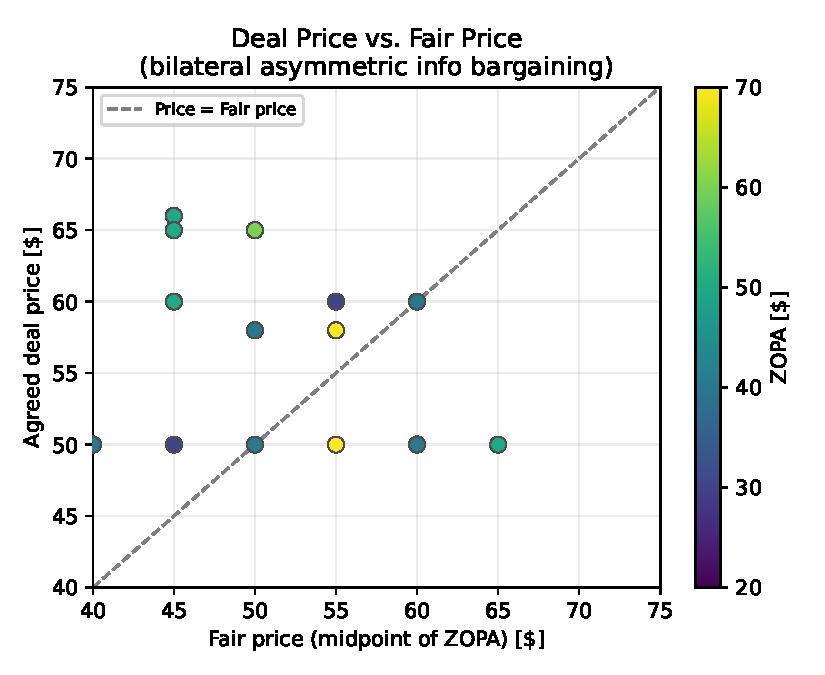
\includegraphics[width=0.55\textwidth]{plots/results_price.pdf}
\caption{Deal price vs.\ fair-price midpoint ($(v+c)/2$) for each session. Points above the dashed diagonal indicate AI-favorable outcomes (price above midpoint). Color encodes ZOPA size. Most points cluster slightly above the diagonal.}
\label{fig:price}
\end{figure}

\subsection*{Surplus Split by Condition (Figure~\ref{fig:surplus})}

The AI (seller) earned a mean of \$25.10 vs.\ \$18.40 for the human (buyer), capturing approximately 55\% of the total surplus on average. A paired $t$-test found the AI advantage to be marginally significant (one-tailed $p = 0.079$). The buyer surplus share was 0.45 (SD $= 0.26$), below the equal-split benchmark of 0.50, though the distribution is wide.

By seller cost: mean deal prices were \$58.00 (sc $=$ \$20), \$51.33 (sc $=$ \$30), \$55.00 (sc $=$ \$40), and \$50.01 (sc $=$ \$50). The negative relationship (higher seller cost $\to$ lower deal price) is counter to theory and is explained by the buyer's anchoring behavior described below.

\begin{figure}[h!]
\centering
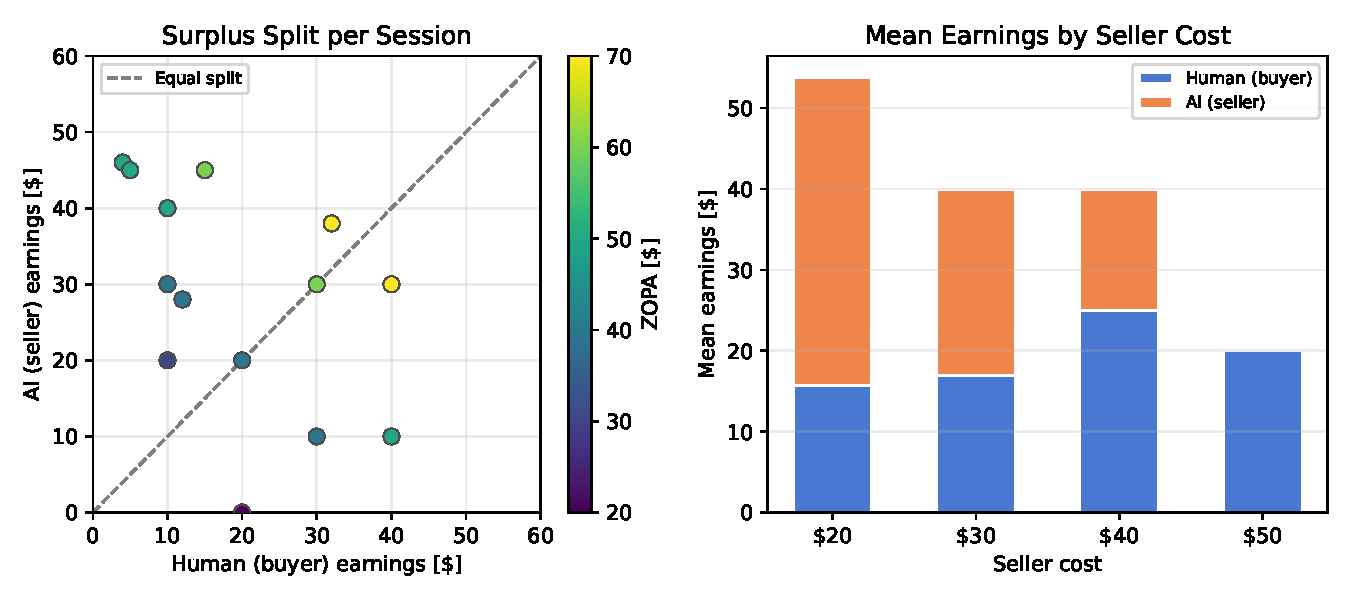
\includegraphics[width=0.85\textwidth]{plots/results_surplus.pdf}
\caption{\textit{Left:} Buyer vs.\ AI earnings per session; dashed line $=$ equal split. \textit{Right:} Mean earnings by seller cost. Error bars omitted due to small cell sizes.}
\label{fig:surplus}
\end{figure}

\subsection*{Parameter Effects and Bargaining Dynamics (Figure~\ref{fig:dynamics})}

\textbf{The most striking finding} is that deal price is nearly unresponsive to the game parameters (OLS regression: $R^2 = 0.14$; buyer-value coefficient $= 0.054$, seller-cost coefficient $= -0.223$). Standard theory predicts that deal prices should increase in seller cost (minimum acceptable price) and increase in buyer value (maximum willingness to pay), producing $R^2$ near 1.0. Neither prediction holds.

The source of this finding is clear from Figure~\ref{fig:dynamics}: the simulated buyer (\texttt{gpt-5-nano}) consistently anchors at \$50.00 as its opening offer. Specifically, 11 of 16 opening offers were exactly \$50.00 and the mean opening offer was \$50.00 (SD $= \$5.00$), \emph{regardless of the buyer's true value} ($v \in \{60, 70, 80, 90\}$). This means a buyer with value $v = 90$ opens at the same price as a buyer with value $v = 60$ --- a massive failure to condition on private information.

Consequence: most negotiations were highly positional. The mode was 5 rounds (14/20 sessions), as the AI repeatedly countered above \$50 and the buyer refused to update. The AI eventually capitulated in Round 5 to avoid the disagreement payoff of \$0. In two sessions with seller cost $= \$50$, the AI accepted at exactly \$50.00 --- earning \$0 --- rather than taking the outside option of \$0. This constitutes a clear AI decision-quality failure.

\begin{figure}[h!]
\centering
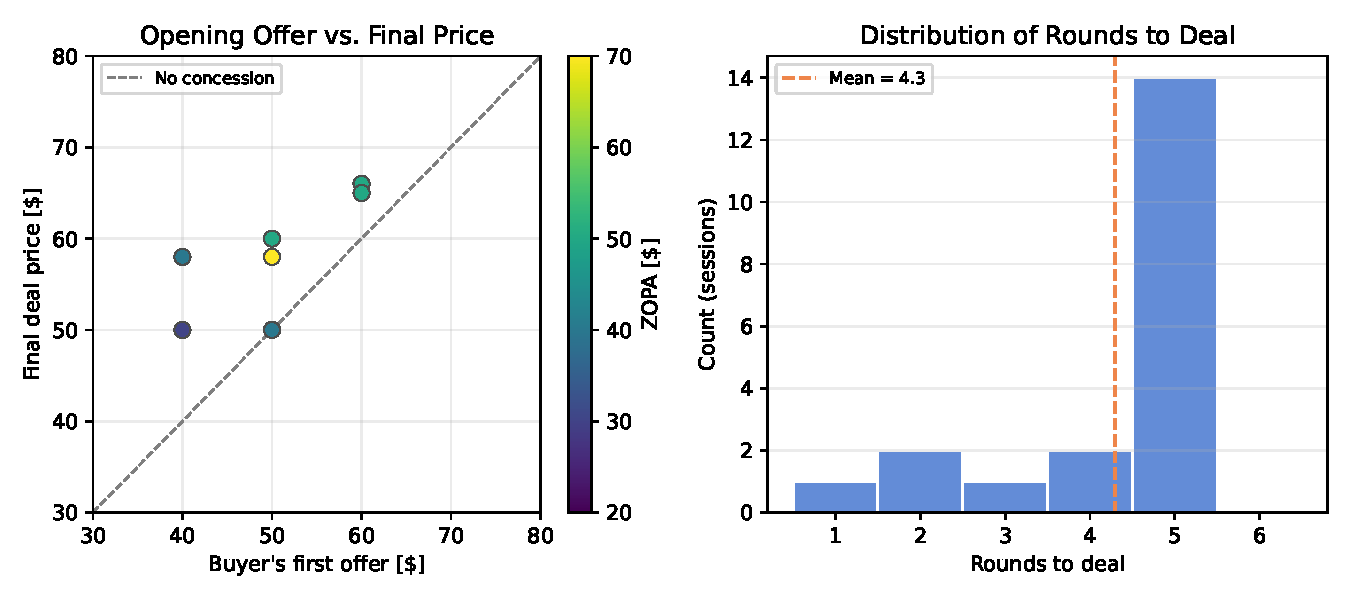
\includegraphics[width=0.85\textwidth]{plots/results_dynamics.pdf}
\caption{\textit{Left:} Buyer's opening offer vs.\ final deal price. Most buyers open at \$50 regardless of their value; final prices vary due to AI concession behavior. \textit{Right:} Distribution of rounds to deal; mode $= 5$, meaning most games go to the final round.}
\label{fig:dynamics}
\end{figure}

%% --- 5. EVALUATION ---
\section*{Evaluation}

\subsection*{Did We Learn Something Interesting?}

\textbf{Partially --- we found a clear behavioral anomaly but the design conflates two sources.}

The interesting finding is: \textbf{the gpt-5-nano buyer anchors rigidly at \$50, failing to condition offers on its private value.} This is not rational information-hiding (a buyer \emph{could} strategically low-ball regardless of value); it appears to be a genuine failure of value-based reasoning by the smaller model. The resulting deal prices are nearly constant (\$50--\$66 range) despite a 4$\times$ variation in ZOPA (\$20--\$70).

However, what we learned is unclear for two reasons:

\begin{enumerate}
\item \textbf{Model conflation.} The buyer uses \texttt{gpt-5-nano} and the AI seller uses \texttt{gpt-5}. The behavioral asymmetry we observe (buyer rigid, AI concedes) could reflect: (a) the gpt-5-nano model's limited strategic capacity, (b) a game design issue in \texttt{sim\_human.md} that anchors the buyer at \$50, or (c) rational buyer strategy. We cannot distinguish without isolating each factor.

\item \textbf{No baseline condition.} We do not know what the same game looks like with symmetric information or with \texttt{gpt-5} on both sides, so we cannot attribute the behavior to the information structure.
\end{enumerate}

Score against the triviality dimensions:
\begin{itemize}
    \item \textit{Surprising?} Yes --- the near-zero price sensitivity ($R^2 = 0.14$) was unexpected.
    \item \textit{Fills a gap?} Partially --- documents LLM bargaining behavior under bilateral asymmetry.
    \item \textit{Mechanism clear?} No --- model vs.\ prompt vs.\ rationality confounded.
    \item \textit{Credible evidence?} Low --- $N = 20$ is small, randomization was unbalanced, no control condition.
\end{itemize}

\subsection*{Limitations}

\begin{itemize}
    \item \textbf{Unbalanced design.} Random draw yielded 9 sessions at $v = 70$ and only 2 at $c = 50$. A factorial design (16 cells, 2--3 reps each) would better identify parameter effects.
    \item \textbf{Buyer model.} The sim\_human uses \texttt{gpt-5-nano}, a smaller model likely less capable of strategic reasoning. The \$50 anchor may reflect this model's limitations rather than the information structure.
    \item \textbf{AI decision quality.} The AI seller accepted a zero-profit deal in 2 sessions ($c = 50$, $p = \$50.00$). This violates rational play. A better AI player prompt should include ``never accept a price that leaves you with zero or negative profit unless all rounds are exhausted.''
    \item \textbf{No baseline.} Without a symmetric-information condition, we cannot attribute deal price patterns to the asymmetric information structure.
\end{itemize}

%% --- 6. NEXT EXPERIMENT ---
\section*{Next Experiment}

\textbf{Archetype: REFINE.} The game design has two issues that prevent clean inference: (1) buyer model (\texttt{gpt-5-nano}) is too weak to reason about private values, and (2) no between-subjects manipulation. The next experiment should run the same bargaining game with \texttt{gpt-5} as both the buyer and seller, and compare symmetric vs.\ asymmetric information conditions to test whether information structure (not model capability) drives the price-insensitivity result.

\textbf{Proposed next experiment:} ``Does bilateral information asymmetry reduce surplus efficiency in LLM bargaining, relative to a symmetric-information baseline?''

\begin{itemize}
    \item \textbf{Condition A (Asymmetric):} Same as current game --- neither side knows the other's value.
    \item \textbf{Condition B (Symmetric):} Both sides know both $v$ and $c$ (full information; both agents calculate the Nash midpoint).
    \item \textbf{Buyer model:} \texttt{gpt-5} for both sides (use \texttt{--model gpt-5} in the sim\_human prompt).
    \item \textbf{Design:} Factorial $2 \times 4 \times 4$ (info $\times$ $v$ $\times$ $c$), at least 2 reps per cell $\Rightarrow N \approx 64$.
    \item \textbf{Primary test:} Does deal price respond to $v$ and $c$ under symmetric info but not asymmetric info?
    \item \textbf{Expected finding:} Under symmetric info, $R^2$ near 1.0 (prices $\approx$ midpoint always); under asymmetric info, lower $R^2$ but similar deal rate. If gpt-5 buyer also anchors at \$50, the anomaly is confirmed as a model artifact; if not, it was a gpt-5-nano limitation.
\end{itemize}

Run: \texttt{/hypothesize iterate bargain\_asymmetric} to formalize this hypothesis, or \texttt{interview simulate bargain\_asymmetric\_gpt5 -n 64 --design factorial} after creating the revised game files.

\subsection*{Prior Experiment Context (Machine-Readable)}
\begin{verbatim}
prior_hypothesis: Under bilateral asymmetric information, LLM bargaining agents
  reach efficient deals and deal prices reflect private values per Bayesian theory.
verdict: PARTIALLY
diagnosis: IMPLEMENTATION
key_finding: 100% deal rate but deal prices show near-zero sensitivity to private
  values (R2=0.14); gpt-5-nano buyer anchors rigidly at $50 regardless of true value.
key_statistic: R2=0.14 for deal_price ~ buyer_value + seller_cost; mean first
  offer = $50 (SD=$5) for buyer_value in {60,70,80,90}
dag_variables: X=information_structure, M=offer_anchoring, Y=deal_price, Z=ZOPA
testable_implications_results: deal_rate_near_100=CONFIRMED,
  price_increases_in_buyer_value=REFUTED, price_increases_in_seller_cost=REFUTED,
  deal_near_fair_price=PARTIALLY_CONFIRMED(p=0.24)
next_archetype: REFINE
proposed_changes: Use gpt-5 for both buyer and seller; add symmetric-information
  baseline condition; use factorial design with 2+ reps per cell (N~64).
next_hypothesis_sketch: Under bilateral asymmetric information, LLM bargainers
  (gpt-5) show lower price sensitivity to private values than under symmetric
  information, revealing the causal role of information structure vs. model capacity.
\end{verbatim}

\end{document}
